% !TeX root = ../../../book.tex

\subsection{可数无限集}\label{sec:section7.6.3}

让我们继续深入到可数无限集的领域。我们将从一个以数学家大卫·希尔伯特 (David Hilbert) 命名的著名思想实验说起。

\subsubsection*{希尔伯特旅馆}

让我们玩一个假想游戏,这会帮助我们理解无限的奇妙之处。

假设我们有一间酒店,这间酒店有无数个房间。这些房间的编号为房间$1$、房间$2$、房间$3$,依此类推。也就是说,这些房间可以用自然数集 $\mathbb{N}$ \emph{索引}。

我们希望能够容纳尽可能多的客人(这样可以赚更多的钱!),而且由于我们的酒店非常豪华和周到,客人们完全愿意在我们要求时搬房间时搬到新的房间。他们只需几分钟时间收拾行李就可以搬到新的房间。

此外,我们还有一套广播系统,可以让我们同时向所有客人传达信息。

\begin{itemize}
    \item 假设所有房间都住满了。这是一个非常繁忙的周末。一个人走进大堂想要一个房间。我们能给他腾出一个房间吗?如果不能,为什么?如果可以,怎么做?\\

          事实证明,我们可以做到!我们只需把所有客人都向后挪一个房间,然后把这位新客人安排到房间 $1$。\\

          不过,关键是要利用我们的广播系统。如果我们不得不去敲\emph{每个}房间的门,告诉他们向后挪一个房间,我们实际上\emph{永远无法完成};我们会花费无尽的时间去敲门和传递信息。\\

          相反,我们可以做以下的公告:
          \begin{quotation}
              各位尊贵的客人请注意:如果您住在房间 $n$,请移至房间 $n+1$。谢谢合作!
          \end{quotation}
          五分钟后,所有客人移动完毕,房间 $1$ 就空出来可以让我们的新客人入住了。\\

          从理论上讲,我们刚刚验证了集合 $\mathbb{N}$ 和集合 $\mathbb{N} \cup \{ \bigstar \}$ 的基数是相同的,无论 $\bigstar$ 是什么。特别地,可以说 $|\mathbb{N}| = |\mathbb{N} \cup \{0\}|$。我们的酒店只有可数的房间,我们已经为每个自然数对应的每个人安排了一个房间,并且还多安排了一个人。\\
    \item 到了第二天,酒店的房间依旧住满了人。假设现在正在举办 Scrabble\footnote{Scrabble 是一款流行的英文拼字游戏。--- 译者注} 大会,来了无数参会者。这些人都佩戴着写有自然数的名牌,比如参会人 $1$、参会人 $2$、参会人 $3$……\\

          我们能容纳下这些人吗?又该如何分配房间和安排当前的住客呢?\\

          事实证明,我们依然可以做到!关键在于腾出一组无限的房间。\\

          同样地,关键在于一次性向\emph{所有}客人发布统一的公告,而不是逐个敲门。\\

          我们知道偶数房间和奇数房间的数量都是无限的,所以我们决定让当前的酒店住客都住进偶数房间,把参加大会的新客人分配到奇数房间。我们通过广播系统向酒店住客发布以下公告:
          \begin{quotation}
              各位尊贵的客人请注意:如果您住在房间 $n$,请移至房间 $2n$。谢谢合作!
          \end{quotation}
          然后,向在大厅等待的大会客人发布以下公告:
          \begin{quotation}
              各位参会嘉宾请注意:如果您的名牌号码是 $n$,请前往房间 $2n - 1$。谢谢!
          \end{quotation}
          五分钟后,所有酒店客人都已经搬好;再过五分钟,所有大会参会者也都找到了自己的房间。完美解决!\\

          从理论上讲,我们已经验证了两个不相交的可数无限集的并集也是可数无限集。具体来说,我们取当前酒店客人的集合 $A$($A$ 是可数无限集)和等待房间的参会者的集合 $B$($B$ 也是可数无限集,且 $A \cap B = \varnothing$),并找到了 $A \cup B$ 和 $\mathbb{N}$ 之间的双射,其中 $\mathbb{N}$ 代表房间的集合。\\
    \item 现在,假设又有一个大会,他们用另一种语言玩 Scrabble,不想跟之前的会议混在一起。我们该怎么安排才能让每个人都有房间呢?\\

          我们可以用同样的方法!就像之前一样,面对一个满员的酒店和一群无穷多等待房间的人。\\
    \item 假如现在有可数无穷多个会议,每个会议都不希望和其他会议混在一起。那该怎么办呢?\\

          幸运的是,酒店会议组织者给每个会议分配了一个自然数,每个会议的成员都戴着写有那个数字的帽子。此外,每个人还被分配了一个自然数,并佩戴相应的徽章。因此,每个人都有两种身份标识:帽子和徽章。比如,我们有会议 $1$ 的第 $1$ 个人,会议 $7$ 的第 $3$ 个人,会议 $8$ 的第 $12$ 个人,等等。\\

          我们怎么重新安排这些人在酒店中的房间呢?这是否可行?如果可行,怎样才能\emph{高效地}做到这一点呢?\\

          这里的问题在于,我们\textbf{不能}一遍又一遍地使用之前的方法。是的,我们可以用这种方法先安排会议 $1$ 的人。完成后,再安排会议 $2$ 的人。依此类推。但我们\textbf{永远无法}安排\emph{所有}会议。就像之前遇到的问题一样,逐个敲开每一个房间的门会花费太长时间;我们需要\emph{一次性向所有人}发送消息。同样地,这里我们需要向所有酒店的客人发送消息,然后再向所有在门外等待的参会者发送消息。我们需要一个关于去哪个房间的通用``公式''。\\

          我们可以从另一个角度来思考,也许会更容易理解。假设你在会议 $x$,并且你是这个会议的参会者 $y$。你急切地想要一个舒适的床来过夜。你想马上知道该去哪个房间。你不想等待所有在你前面的参会者一一被分配房间。你希望所有人能一次性进入酒点并找到各自的房间。\\

          这是其中一种方法。我们可以利用\emph{质数}的特性。我们知道质数有可数无穷多个,并且对于任意两个\emph{不同的}质数 $p$ 和 $q$(即 $p \ne q$),对于任意自然数 $k$,都有 $p^k \ne q^k$。基于这一点,我们可以将对应质数幂次的房间分配给每个客人,这样可以确保没有两个(潜在的)客人被分配到同一个房间。我们向当前酒店住客发布以下公告:
          \begin{quotation}
              各位尊贵的客人请注意:如果您住在房间 $n$,请移至房间 $2^n$。谢谢合作!
          \end{quotation}
          然后,向等在门外的参会者发布以下公告:
          \begin{quotation}
              各位参会嘉宾请注意:

              如果您是会议 $1$ 的参会者 $k$,请前往房间 $3^k$。

              如果您是会议 $2$ 的参会者 $k$,请前往房间 $5^k$。

              如果您是会议 $3$ 的参会者 $k$,请前往房间 $7^k$。

              也就是说,如果您是会议 $n$ 的参会者 $k$,您的房间号为第 $(n+1)$ 个质数的 $k$ 次幂。

              谢谢合作!
          \end{quotation}
          (注意:我们假设所有的客人都是数学天才,他们可以迅速算出第 $(n + 1)$ 个质数的 $k$ 次幂。否则,我们可能不会希望他们入住我们这间豪华的数学酒店!)\\

          请注意,这样的安排确保了\emph{每个人}都有一个独立的房间,没有人需要与他人共享。不过,这也导致许多房间\emph{空置}。谁住在房间 $1$?谁住在房间 $6$?谁住在房间 $18$?总体来说,你能描述出哪些房间会空置吗?\\

          我们怎样才能更``高效地''利用这些房间呢?是否有某种方法可以让\emph{所有}房间都住满?\\

          从理论上讲,我们刚刚验证了 $\mathbb{N}$ 和 $\mathbb{N} \times \mathbb{N}$ 具有相同的基数。我们有无数个会议,每个会议有无数的参会者,因此我们想要每个人都可以用一个\emph{自然数的有序对}来表示,其中第一个数是人员编号,第二个数是会议编号。既然我们能够将这组人匹配到房间集合(对应 $\mathbb{N}$),那么我们就证明了 $\mathbb{N} \times \mathbb{N}$ 是可数的。(注意:我们实际上``做过头了'',找到了将集合 $\mathbb{N} \times \mathbb{N}$ 嵌入 $\mathbb{N}$ 的\emph{真子集}的方法!)\\
\end{itemize}

希望这能让你了解如何思考可数无穷。一个重要的点是要记住,在这里,\textbf{无穷}是一个\textbf{基数},而不是一个\textbf{数字}。这并不是说自然数会一直延续,并且在它们之后有一个神奇的数字 $\infty$。这里我们把可数\emph{无穷}看作一个\textbf{基数};它代表了某物有多``庞大''。它更像是一个\emph{量级}而不是一个\emph{位置}。

\subsubsection*{示例}

让我们把\textbf{希尔伯特旅馆}示例中传达的一些想法用更正式的方式表达出来。我们将使用单射、满射和双射等概念。以下结论在我们接下来的讨论中会非常有用,因此我们现在就来证明它。

\begin{lemma}\label{lemma7.6.11}
    设 $S, T$ 为任意集合。假设 $S \subseteq T$。则 $|S| \le |T|$。
\end{lemma}

\begin{proof}
    定义``恒等函数'' $f : S \to T$ 为 $\forall x \in S \centerdot f(x) = x$。因为 $S \subseteq T$,因此这是一个良好定义的函数。

    (注意:我们不能严格地将其定义为通常的恒等函数 $\id_S$,因为定义域和值域可能不是同一个集合;本质上,$f$ 执行与 $\id_S$ 相同的操作,但值域不同。)

    显然 $f$ 为单射。

    (注意:$f$ 未必是双射,因为可能 $S \ne T$。)

    因为 $f$ 为单射,这告诉我们 $|S| \le |T|$。
\end{proof}

你可能会想,为什么我们不能在这里得出 $|A| < |B|$ 的结论,而是 ``$\le$'' 呢?确实,对于有限集来说,$\{1, 2\} \subseteq \{1, 2, 3\}$,并且 $|\{1, 2\}| = 2 < 3 = |\{1, 2, 3\}|$。然而,正如我们将在本节中看到的,有些\textbf{无限集}的\emph{真子集}与其本身具有相同的基数!\\

\begin{example}[$\mathbb{Z}$ 是可数无限集]\label{ex:example7.6.12}

    我们知道,根据定义,$\mathbb{N}$ 是可数无限集。恒等函数 $\id_{\mathbb{N}} : \mathbb{N} \to \mathbb{N}$ 显然是一个双射,因此 $\mathbb{N}$ 是可数的。

    在这个例子中,我们将证明 $\mathbb{Z}$ 也是可数无限集!为此,我们需要找到一个双射 $f : \mathbb{Z} \to \mathbb{N}$。我们会在这里提供一个例子,并通过找到它的\emph{反函数}来证明它是一个双射。在继续阅读之前,不妨自己尝试找找看!也许你会想到一个不同的函数!如果需要提示,可以考虑以下思路:为了证明一个无限集是\emph{可数}无限集,我们需要找到一种方法,将元素一个接一个地\emph{列出来}。试着找到一个模式,确定``第一个''整数,然后是``第二个'',接着是``第三个''……

    让我们定义函数 $f : \mathbb{Z} \to \mathbb{N}$ 并通过找到它的反函数 $f^{-1}$ 来证明 $f$ 为双射。

    \begin{proofs}{证明双射:}
        我们选择定义 $f : \mathbb{Z} \to \mathbb{N}$ 为
        \[\forall z \in \mathbb{Z} \centerdot f(z) = \begin{cases}
                -2z + 2          & \text{如果}\; z \le 0 \\
                \enspace\; 2z -1 & \text{如果}\; z > 0
            \end{cases}\]
        我们之所以选择这个函数是因为它可以将整数与自然数进行如下``配对'':
        \begin{center}
            \begin{tabular}{ccccccccc}
                \dots , & -3,            & -2,            & -1,            & 0,             & 1,             & 2,             & 3,             & \dots \\
                        & $\updownarrow$ & $\updownarrow$ & $\updownarrow$ & $\updownarrow$ & $\updownarrow$ & $\updownarrow$ & $\updownarrow$ &       \\
                \dots , & 8,             & 6,             & 4,             & 2,             & 1,             & 3,             & 5,             & \dots
            \end{tabular}
        \end{center}
        (也就是说,我们将偶数与非正整数配对,将奇数与正整数配对。通过观察这种对应关系,我们可以理解如何``逆转''它。这就是我们找到函数 $f$ 的反函数的方法。)

        接着定义函数 $F : \mathbb{N} \to \mathbb{Z}$ 为
        \[F(n) = \begin{cases}
                -\frac{n}{2} + 1 & \text{如果}\; n \;\text{为偶数} \\
                \frac{n+1}{2}    & \text{如果}\; n \;\text{为奇数}
            \end{cases}\]
        我们来证明 $F=f^{-1}$。给定 $z \in \mathbb{Z}$。我们有两种情况:
        \begin{itemize}
            \item 假设 $z > 0$。则 $f(z)=2z-1$。显然 $2z-1 \in \mathbb{N}$ 且 $2z-1$ 为奇数。这意味着
                  \[(F \circ f)(z) = F(f(z)) = F(2z - 1) = \frac{(2z-1)+1}{2} = \frac{2z}{2} = z\]
            \item 假设 $z \le 0$。则 $f(z)=-2z+2$。显然 $-2z \ge 0$,所以 $-2z + 2 \ge 2$,因此 $-2z + 2 \in \mathbb{N}$ 且 $-2z + 2$ 为偶数。这意味着
                  \begin{align*}
                      (F \circ f)(z) & = F(f(z)) = F(-2z + 2) = \frac{-2z + 2}{2}+1 \\
                                     & = -(-z + 1) + 1 = (z - 1) + 1 = z
                  \end{align*}
        \end{itemize}
        无论哪种情况,都得到 $(F \circ f)(z) = z$。这表明 $F \circ f = \id_{\mathbb{Z}}$。\\

        接下来,设 $n \in \mathbb{N}$。我们有两种情况:
        \begin{itemize}
            \item 假设 $n$ 为偶数。则 $F(n) = -\frac{n}{2} + 1$。显然 $\frac{n}{2} \ge 1$,所以 $-\frac{n}{2} + 1 \le -1+1=0$。这意味着
                  \begin{align*}
                      (f \circ F)(n) & = f(F(n)) = f\Big(-\frac{n}{2}+1\Big) = -2\Big(-\frac{n}{2}+1\Big)+2 \\
                                     & = \Big(\frac{2n}{2}-2\Big)+2=n
                  \end{align*}
            \item 假设 $n$ 为奇数。则 $F(n) = \frac{n+1}{2}$。显然 $n+1 \ge 2$,所以 $\frac{n+1}{2} \ge 1$。这意味着
                  \begin{align*}
                      (f \circ F)(n) & = f(F(n)) = f\Big(\frac{n+1}{2}\Big) = 2(\frac{n+1}{2}\Big)-1 = \frac{2n+2}{2}-1 \\
                                     & = (n + 1) -1 = n
                  \end{align*}
        \end{itemize}
        无论哪种情况,都得到 $(f \circ F)(n) = n$。这表明 $f \circ F = \id_{\mathbb{N}}$。\\

        因此 $F = f^{-1}$。
    \end{proofs}
\end{example}

这表明 $\mathbb{Z}$ 和 $\mathbb{N}$ 具有相同的基数,即 $|\mathbb{Z}| = |\mathbb{N}|$。你可能会觉得整数的数量是自然数的``两倍'',但这其实是一个误解。我们可以将这两个集合的元素\emph{一一对应},所以它们的大小是相同的!这个例子说明了为什么引理 \ref{lemma7.6.11} 的结论是正确的。在这里,虽然 $\mathbb{N} \subset \mathbb{Z}$($\mathbb{N}$ 是 $\mathbb{Z}$ 的真子集),但 $|\mathbb{N}| = |\mathbb{Z}|$。这种情况只有在集合是无限集的情况下才会发生,这就是一个例子。

(在本节后面,我们将\emph{证明}这是判定集合是否为无限集的一种等价方法:即能否找到集合与其真子集之间的双射。)\\

\begin{example}[$\mathbb{N} \times \mathbb{N}$ 是可数无限集]\label{ex:example7.6.13}

    在上一节关于\textbf{希尔伯特旅馆}的讨论中,我们基本上论证了 $\mathbb{N} \times \mathbb{N}$ 与 $\mathbb{N}$ 具有相同的基数。当我们有无穷多个会议,每个会议都有无穷多人时,我们仍然可以将他们全部安置在拥有无穷多间客房的酒店里!不过那只是一个直观的讨论,所以现在我们来正式证明这一事实。我们将找到这两个集合之间的一个\emph{双射}函数。我们将证明它是满射,并请你帮忙证明它是单射。

    \begin{proofs}{证明双射:}
        定义函数 $f : \mathbb{N} \times \mathbb{N} \to \mathbb{N}$ 为
        \[\forall (x, y) \in \mathbb{N} \times \mathbb{N} \centerdot f(x, y) = 2^{x-1}(2y - 1)\]
        在证明 $f$ 为双射的过程中,我们实际上要证明如下事实:
        \begin{quotation}
            所有自然数都可以\emph{唯一地}写成 $2$的幂乘以一个奇数的形式。
        \end{quotation}
        我们来看一下我们定义的这个函数。它接受一对自然数,并输出 $2$ 的幂乘以一个奇数。证明这个函数是双射函数意味着它不会输出相同的自然数(单射性),并且每个自然数都可以由某对输入得到(满射性)。你可以尝试使用这个函数,输入一些值看看结果。另外,你也可以尝试``逆向''思考,看看 $f^{-1}$ 会怎样。例如,选择一个你喜欢的 $n \in \mathbb{N}$。你能把它表示为 $2$ 的幂乘以一个奇数吗?如果 $n$ 为奇数,这很简单,因为 $2^0 = 1$。例如:
        \[11 = 1 \cdot 11 = 2^0 \cdot (2 \cdot 6 - 1) = f(1, 6)\]
        (注意:在定义函数时我们不得不使用 $x - 1$ 和 $2y - 1$ 是因为我们的定义域和值域都涉及 $\mathbb{N}$,而 $0 \notin \mathbb{N}$。)

        如果 $n$ 为偶数,我们可以不断地将其除以 $2$,直到不能再除为止;剩下的必定是奇数。例如:
        \begin{align*}
            40 & = 2 \cdot 20 = 4 \cdot 10 = 8 \cdot 5 = 2^3 \cdot (2 \cdot 3 - 1) = f(4, 3)                        \\
            32 & = 2 \cdot 16 = 2^2 \cdot 8 = 2^3 \cdot 4 = 2^4 \cdot 2 = 2^5 = 2^5 \cdot (2 \cdot 1 - 1) = f(6, 1)
        \end{align*}
        这一洞察对证明 $f$ 是满射至关重要。\\

        $f$ \textbf{为单射}:我们声称 $\forall n \in \mathbb{N} \centerdot n \in Im_f (\mathbb{N} \times \mathbb{N})$。我们通过``最小罪犯''论证来证明这一点。

        \textbf{基本情况}:易得 $f(1, 1) = 2^0 \cdot 1 = 1$。因此,$1 \in Im_f (\mathbb{N} \times \mathbb{N})$。

        \textbf{归纳假设}:假设我们有 $n \in \mathbb{N} - \{1\}$ 不能写成 $2$ 的幂乘以一个奇数的形式,即假设 $n \notin Im_f (\mathbb{N} \times \mathbb{N})$。

        \textbf{归纳步骤}:我们有两种情况:
        \begin{itemize}
            \item 如果 $n$ 为奇数,则 $n \cdot 2^0 = n \cdot 1 = n$ 就是这种表达形式。也就是说,我们知道 $\frac{n+1}{2} \in \mathbb{N}$ 且我们发现
                  \[f\Big(1, \frac{n+1}{2}\Big) = 2^0 \cdot \Big(2 \cdot \frac{n+1}{2}-1\Big) = 1 \cdot (n + 1 - 1) = n\]
                  所以 $n \in Im_f (\mathbb{N} \times \mathbb{N})$。这与我们的假设 $n \notin Im_f (\mathbb{N} \times \mathbb{N})$ 矛盾。所以这种情况不成立。
            \item 如果 $n$ 为偶数,则考虑 $\frac{n}{2}$。为了引出矛盾而假设 $\frac{n}{2}$ 可以写成 $2$ 的幂乘以一个奇数的形式,即假设 $\frac{n}{2} \in Im_f (\mathbb{N} \times \mathbb{N})$。这意味着 $\exists (x, y) \in \mathbb{N} \times \mathbb{N} \centerdot f(x, y) = \frac{n}{2}$。给定这样的 $(x,y)$。然后考虑 $f(x + 1, y)$(这是有效的,因为 $x+1 \in \mathbb{N}$)。我们发现
                  \[f(x + 1, y) = 2^{x+1} \cdot (2y - 1) = 2 \cdot \big(2^x \cdot (2y - 1)\big) =  2 \cdot f(x, y) = 2 \cdot \frac{n}{2} = n\]
                  这表明 $n$ 也有这种表达形式,即 $n \in Im_f (\mathbb{N} \times \mathbb{N})$。而这再一次与我们的假设 $n \notin Im_f (\mathbb{N} \times \mathbb{N})$ 矛盾。因此 $\frac{n}{2}$ 不具有这种表达形式,即 $\frac{n}{2} \notin Im_f (\mathbb{N} \times \mathbb{N})$。
        \end{itemize}

        我们已经证明,如果假设 $n$ 是该命题的一个反例,那么 $\frac{n}{2}$ 将是一个\emph{更小的}反例。通过``最小罪犯''论证法(因为我们已经证明了基本情况),我们可以得出结论,该命题对所有 $n \in \mathbb{N}$ 都成立。这说明 $f$ 满射。
    \end{proofs}

    (注意:你可能需要回顾 \ref{sec:section5.5.1} 节,以重新理解``最小罪犯''论证的工作原理。)

    $\mathbf{f}$ \textbf{为满射}:留作练习 \ref{exc:exercises7.8.21} 由你来证明。

    综上,我们已经证明 $f$ 为双射,因此 $|\mathbb{N} \times \mathbb{N}| = |\mathbb{N}|$。也就是说,$\mathbb{N} \times \mathbb{N}$,即所有自然数有序对的集合是可数无限集。这让你感到惊讶吗?这是否有些违反直觉?你觉得所有自然数有序\emph{三元组}的集合 $\mathbb{N}^3$ 会是什么样的呢?如果我们继续考虑 $\mathbb{N} \times \mathbb{N} \times \mathbb{N} \dots$ 会发生什么呢?思考这些问题,与同学们讨论一下,并尝试证明一些结论吧!
\end{example}

\begin{example}[$\mathbb{N} \times \mathbb{N}$ 格]\label{ex:example7.6.14}

    在进入下一个例子之前,我们再来看看 $|\mathbb{N} \times \mathbb{N}| = |\mathbb{N}|$ 的另一种解释。这次我们用一种更直观的方式来说明,虽然不进行正式定义,但可以帮助你理解如何在这两个集合之间建立双射。这种解释很常见,也很值得一看。

    这个思路是将 $\mathbb{N} \times \mathbb{N}$ 想象成一个二维正方形\emph{格 (Lattice)}\footnote{格是一个数学概念。在数学中,格是其非空有限子集都有一个上确界(叫并)和一个下确界(叫交)的偏序集合(poset)。最常见的二维格由平面上所有整点组成,也就是说,这些点在直角坐标系里的横纵坐标都是整数。我们称这种格为``正方形格''。--- 译者注},如下所示:

    \begin{center}
        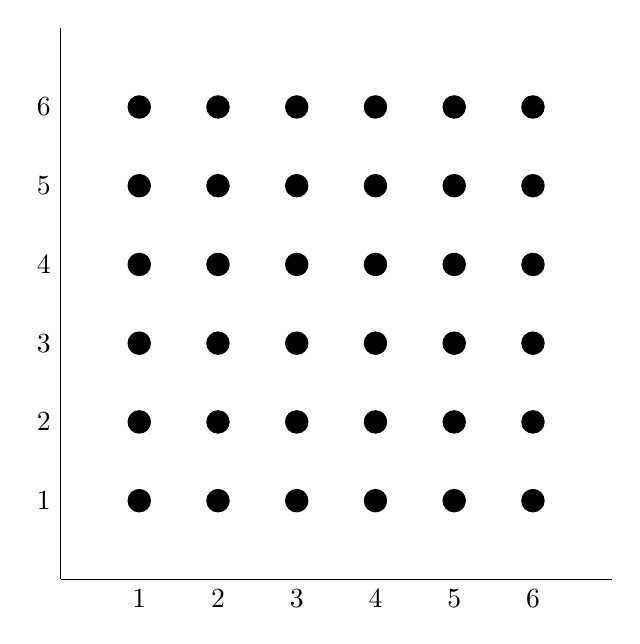
\begin{tikzpicture}[scale=1]
            \foreach \x in {1,...,6}
                {
                    \foreach \y in {1,...,6}
                        {
                            \node at (\x, \y)[circle,fill,inner sep=3pt]{};
                        }
                    \node[left] at (0, \x){$\x$};
                    \node[below] at (\x, 0){$\x$};
                }

            \draw (0.0, 0.0) -- (7.0, 0.0);
            \draw (0.0, 0.0) -- (0.0, 7.0);
        \end{tikzpicture}
    \end{center}

    为了证明这个格上无限多顶点是\textbf{可数}无限的,我们可以描述一条路径,该路径遍历所有的点(满射!)且每个点只遍历一次(单射!),并用自然数进行索引(可数无限!)。也就是说,我们可以描述一种通过一系列步骤遍历整个格上顶点的方式;会有一个``第一个点''和一个``第二个点''等等。

    关键的洞察是,这个格的左上对角线都是\textbf{有限的}。例如,从点 $(5, 1)$ 开始,向左上对角移动。你将经过 $(4, 2), (3, 3), (2, 4), (1, 5)$,然后到达格的边界。不论你从底部的哪一行开始,这都是正确的。

    让我们利用这一事实,根据 (a) 它所在的对角线,以及 (b) 它在该对角线上的位置,用自然数标记每个点。我们将从 $(1, 1)$ 开始的对角线视为第一条对角线,将从 $(2, 1)$ 开始的对角线视为第二条对角线,依此类推。这给了我们以下标注:

    \begin{center}
        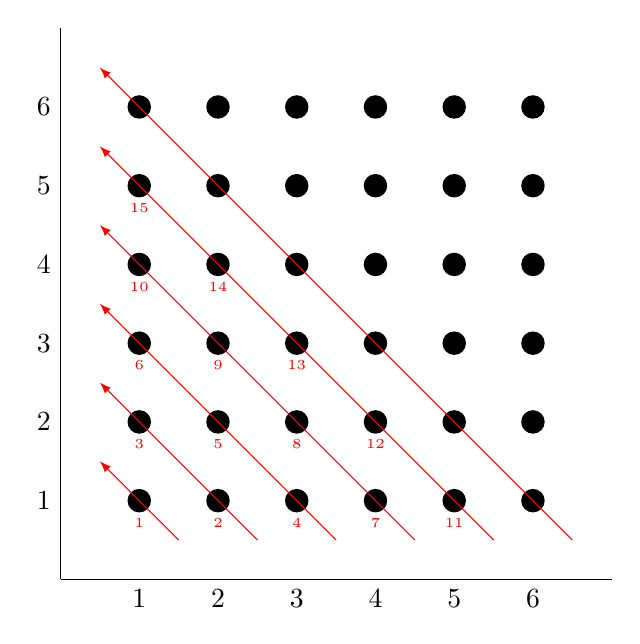
\begin{tikzpicture}[scale=1]
            \foreach \x in {1,...,6}
                {
                    \foreach \y in {1,...,6}
                        {
                            \node at (\x, \y)[circle,fill,inner sep=3pt]{};
                        }
                    \node[left] at (0, \x){$\x$};
                    \node[below] at (\x, 0){$\x$};
                    \draw[-latex, red] (\x+0.5, 0.5) -- (0.5, \x+0.5);
                }

            \draw (0.0, 0.0) -- (7.0, 0.0);
            \draw (0.0, 0.0) -- (0.0, 7.0);

            \foreach \y / \t in {1/1, 2/3, 3/6, 4/10, 5/15}
                {
                    \node[below,red] at (1, \y-0.1){\tiny$\t$};
                }
            \foreach \y / \t in {1/2, 2/5, 3/9, 4/14}
                {
                    \node[below,red] at (2, \y-0.1){\tiny$\t$};
                }
            \foreach \y / \t in {1/4, 2/8, 3/13}
                {
                    \node[below,red] at (3, \y-0.1){\tiny$\t$};
                }
            \foreach \y / \t in {1/7, 2/12}
                {
                    \node[below,red] at (4, \y-0.1){\tiny$\t$};
                }
            \node[below,red] at (5, 0.9){\tiny$11$};

        \end{tikzpicture}
    \end{center}

    我们可以看到,格中的每个顶点都会恰好落在某条对角线上。此外,这些对角线的数量是可数无限的(由 $\mathbb{N}$ 索引),而每条对角线上只有\emph{有限}多个点。这意味着(我们将在下面证明)所有对角线上的点的集合是可数无限集。

    你可以尝试通过定义一个函数来实现我们展示的标记方法,从而\emph{形式化}这个论点。或者,你也可以使用类似的方法,比如向右下方向移动,或者交替反转对角线的方向……
\end{example}

\begin{example}[$\mathbb{Q}$ 是可数无限集]

    这个结果是我们在处理无限集及其基数时,直觉失灵的一个显著例子。想象一下,把 $\mathbb{Q}$ 的元素分布在数轴上。它们似乎无处不在!事实上,回看练习 \ref{exc:exercises4.11.26},在那道练习中,你证明了有理数是\textbf{稠密的},这意味着在 $\mathbb{R}$ 中也是如此(即任意两个不同实数之间都存在一个有理数)。此外,有理数集\emph{看起来}比整数集 $\mathbb{Z}$ 大得多:仅在 $0$ 和 $1$ 之间,就有无穷多个有理数!出于这些原因,你可能会认为 $\mathbb{Q}$ 是不可数无限集,但这是错误的。

    在这个例子中,我们将提供几个论证来证明这一点,因为我们意识到这个结论确实非常奇特和炸裂。

    \begin{enumerate}[label=(\arabic*)]
        \item \textbf{直观解释:}\\
              考虑以下将 $\mathbb{Q}$ 表示为集合并集的形式:
              \[\mathbb{Q} \;\text{``}=\text{''}\; \big(\text{``}\mathbb{N} \times \mathbb{N}\text{''}\big) \cup \big(\text{``}-(\mathbb{N} \times \mathbb{N})\text{''}\big) \cup \{0\}\]
              某种意义上,$\mathbb{N} \times \mathbb{N}$ 可以对应所有正有理数。要理解这一点,只需考虑函数 $f : \mathbb{N} \times \mathbb{N} \to \mathbb{Q}_+$,定义为 $f(x, y) = \frac{x}{y}$。这个函数确实能够生成所有正有理数(因此 $f$ 是一个满射),但由于 $\frac{4}{2}=\frac{2}{1}$,所以它不是一个单射。因为 $f$ 是满射,这至少表明 $|\mathbb{N} \times \mathbb{N}| \ge |\mathbb{Q}|$。由于 $\mathbb{N} \times \mathbb{N}$ 是可数无限集,而 $\mathbb{Q}$ 显然也是无限集,这表明正有理数是可数无限集。\\

              负有理数集 $\mathbb{Q}_-$ 也具有与正有理数集 $\mathbb{Q}_+$ 相同的基数。它们之间存在明确的双射关系:定义函数 $g : \mathbb{Q}_+ \to \mathbb{Q}_-$ 为 $\forall q \in \mathbb{Q}_+ \centerdot g(q) = -q$。\\

              这里唯一遗漏的是 $0 \in \mathbb{Q}$。两个可数无穷集的并集仍然是可数无穷集(我们将在下面证明),再加上一个元素也不会改变这一点。因此,$\mathbb{Q}$ 是可数无限集。\\

              需要注意的是,这里有点``随意''。上面``等式''中的所有``引号''表示你应该仅将其作为启发性论证,而不是严格证明。然而,确实有方法可以使这些论证形式化。试着自己动手做做看吧!\\
        \item \textbf{列出 $\mathbb{Q}$ 中元素:}\\
              考虑编写一个计算机程序,列出所有正有理数。你会使用什么算法?只要你能保证你的程序``最终''会成功列出所有这些数,那么你就已经证明了 $\mathbb{Q}$ 可以一个一个地枚举出来,因此它必然是可数无限集。(这也是为什么我们使用 $\mathbb{N}$ 作为典型的可数无限集:我们可以一个一个地枚举它的元素,我们可以数它们。)\\

              这里有一种方法可以编写该程序:按照我们在前一个例子中使用 $\mathbb{N} \times \mathbb{N}$ ``格点路径''论证。这次,只需``跳过''已经打印过的有理数。\\

              也就是说,我们会先打印 $(1, 1) \leftrightarrow 1$,然后是 $(2, 1) \leftrightarrow 2$,再然后是 $(1, 2) \leftrightarrow \frac{1}{2}$,接着是 $(3, 1) \leftrightarrow 3$,依此类推……\\

              哦!我们需要跳过 $(2, 2) \leftrightarrow 1$。我们怎么知道的?因为我们已经打印过 $1$。我们怎么知道某个数已经打印过了?我们只需查看已经打印过的有理数列表,检查即将打印的数是否已经出现过。如果已经出现过,就跳过;如果没有,就打印它然后继续。\\

              在枚举过程中,这意味着对于我们经过的每个格点,我们只需检查\emph{有限的}项;也就是说,我们需要查看已经打印过的\emph{有限大的}有理数集合。这意味着在每一步打印过程中会花费``稍长一点的时间'',但不会\emph{无限长}。因此,我们的程序最终会列出每一个有理数;无论你想到的是哪个,我们都会在有限的时间内到达它。\\
        \item \textbf{$\mathbb{Q}$ 至多是可数无限集:}\\
              这是 $\mathbb{Q}$ 是可数集的另一个论证。(如果你觉得有点多余,那也没关系,可以跳过。我们只是觉得这个结果很有趣,从多个角度思考问题可能会有所帮助!)\\

              请思考一下:我们可以先验地认为 $|\mathbb{Q}| \ge |\mathbb{N}|$。这是因为 $\mathbb{Q} \supseteq \mathbb{N}$。现在,唯一的问题是这些基数是否相等。为了得出这个结论,我们需要找到
              \begin{enumerate}[label=(\alph*)]
                  \item 从 $\mathbb{Q}$ 到某个可数集的单射;
                  \item 从某个可数集到 $\mathbb{Q}$ 的满射。\\
              \end{enumerate}

              我们将在下面证明 $\mathbb{Z} \times \mathbb{N}$ 是可数的。(也就是说,我们将证明任意两个可数无限集的笛卡尔积也是可数无限集。)然后我们可以定义函数 $f : \mathbb{Z} \times \mathbb{N} \to \mathbb{Q}$ 为
              \[\forall (z, n) \in \mathbb{Z} \times \mathbb{N} \centerdot f(z, n) = \frac{z}{n}\]
              该函数是 $\mathbb{Q}$ 上的满射。虽然它肯定不是单射(为什么不是?)但这并不影响我们的结论。它表明 $|\mathbb{Z} \times \mathbb{N}| = |\mathbb{Q}|$。一旦我们证明了 $|\mathbb{Z} \times \mathbb{N}| = |\mathbb{N}|$,就可以得出 $|\mathbb{N}| = |\mathbb{Q}|$。\\
        \item \textbf{Stern-Brocot 树:}\\
              $\mathbb{Q}$ 还有其他视觉表示方法,其中 \textbf{Stern-Brocot 树}尤其具有启发性。这个概念最早由法国钟表匠 Achille Brocot 提出并发展,他在制作钟表时需要找到齿轮齿数的近似值。大约在同一时期($19$ 世纪 $50$ 年代和 $60$ 年代),德国数学家 Moritz Stern 也发展了这一想法。令人惊讶的是,一位非数学家竟然能\emph{独立地}发展出这样一个迷人的概念来解决实际问题!\\

              (不必过于担心\emph{图}和\emph{树}等术语。我们不会深入讨论它们,只是简单介绍一下,帮助理解 $\mathbb{Q}$ 的表示方法,并展示它是可数无穷集。)\\

              这棵树的\textbf{根节点}为 $1$。(即图中最顶端的数字。)\textbf{父节点和子节点的关系}(即如何生成树的下一层节点)是通过连分数定义的。(我们在这里不详细解释其含义,而是描述如何构建这棵树。)\\

              通过这种构造方法,从根节点到任一节点的路径会产生一系列有理数,这些有理数逐渐逼近最终的节点。此外,序列中的每个后续有理数的分母都比前一个大。这正是 Brocot 先生的动机所在。他需要确定手表内部两个齿轮的齿数,使它们的大小比率非常接近某个特定数值。通过沿着这棵树向下寻找,他可以找到更接近所需数值的近似比率!是不是很酷?

              \begin{center}
                  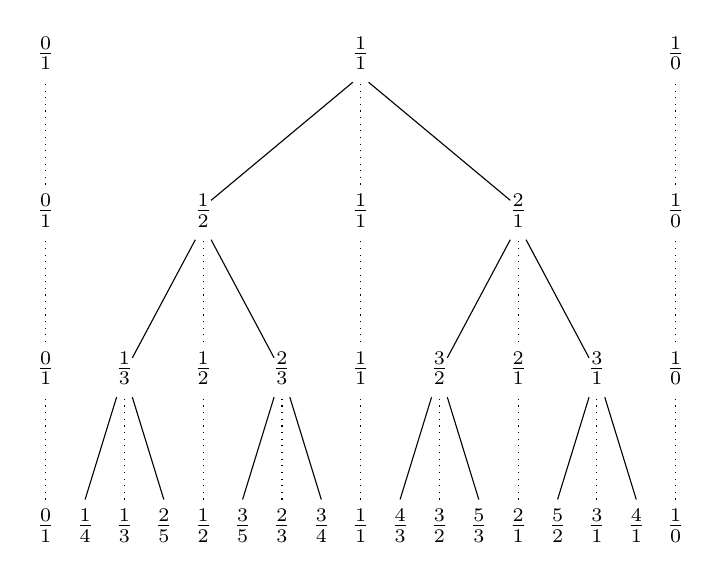
\begin{tikzpicture}[scale=1]
                      \edef \step {0.5};
                      \foreach \a / \b in {1/4, 1/3, 2/5, 1/2, 3/5, 2/3, 3/4}
                          {
                              \node[below] at (\step, 0){$\frac{\a}{\b}$};
                              \node[below] at (8-\step, 0){$\frac{\b}{\a}$};
                              \pgfmathparse{\step + 0.5};
                              \xdef \step{\pgfmathresult};
                          }

                      \edef \step {1.0};
                      \foreach \a / \b in {1/3, 1/2, 2/3}
                          {
                              \node[below] at (\step, 2){$\frac{\a}{\b}$};
                              \node[below] at (8-\step, 2){$\frac{\b}{\a}$};
                              \pgfmathparse{\step + 1.0};
                              \xdef \step{\pgfmathresult};
                          }

                      \node[below] at (2, 4){$\frac{1}{2}$};
                      \node[below] at (6, 4){$\frac{2}{1}$};

                      \foreach \y in {0,...,3}
                          {
                              \node[below] at (0, \y*2){$\frac{0}{1}$};
                              \node[below] at (4, \y*2){$\frac{1}{1}$};
                              \node[below] at (8, \y*2){$\frac{1}{0}$};
                          }

                      \edef \mx {0.1};
                      \edef \mya {0.2};
                      \edef \myb {0.7};
                      \foreach \y in {0,...,2}
                          {
                              \draw[dotted] (4, \y*2) -- (4, \y*2 + 2-\myb);
                          }

                      \foreach \x in {0,...,3}
                          {
                              \draw[dotted] (\x, 0.0) -- (\x, 2-\myb);
                              \draw[dotted] (8-\x, 0.0) -- (8-\x, 2-\myb);
                              \draw (\x*2+0.5, 0.0) -- (\x*2+1-\mx, 2-\myb);
                              \draw (\x*2+1.5, 0.0) -- (\x*2+1+\mx, 2-\myb);
                          }
                      \foreach \x in {0,...,1}
                          {
                              \draw[dotted] (\x*2, 2.0) -- (\x*2, 4-\myb);
                              \draw[dotted] (8-\x*2, 2.0) -- (8-\x*2, 4-\myb);
                              \draw (\x*4+1+\mx, 2.0-\mya) -- (\x*4+2-\mx, 4-\myb);
                              \draw (\x*4+3-\mx, 2.0-\mya) -- (\x*4+2+\mx, 4-\myb);
                          }
                      \foreach \x in {0}
                          {
                              \draw[dotted] (\x*8, 4.0) -- (\x*8, 6-\myb);
                              \draw[dotted] (8-\x*8, 4.0) -- (8-\x*8, 6-\myb);
                              \draw (\x*8+2+\mx, 4.0-\mya) -- (\x*8+4-\mx, 6-\myb);
                              \draw (\x*8+6-\mx, 4.0-\mya) -- (\x*8+4+\mx, 6-\myb);
                          }
                  \end{tikzpicture}
              \end{center}

              为了实际\emph{构建}这棵树,我们需要找到\emph{中位数}。给定两个有理数 $\frac{a}{b}$ 和 $\frac{c}{d}$,它们的中位数定义为 $\frac{a+b}{c+d}$。(注意,这里的中位数指的是一种特殊的对象;这\emph{不是}两个分数相加的正确方法!)\\

              树的每一层由上一层中相邻有理数对的所有中位数组成;我们不``计算''直接垂直的元素,它们只是为了便于阅读和构建而保留的。此外,注意分数 $\frac{0}{1}$ 和 $\frac{1}{0}$(尽管 $\frac{1}{0}$ 是未定义的!)包含在外侧列中,用于辅助生成每层最外侧的元素。\\

              (可以尝试探索这棵树的性质,并阅读更多\href{https://en.wikipedia.org/wiki/Stern%E2%80%93Brocot_tree}{相关内容}。这是一个非常有趣的数学对象!)\\

              我们在这里不会证明这棵树包含\emph{所有}有理数,但我们相信你可以理解为什么这是可信的。此外,我们也相信你可以理解为什么这棵树中的所有节点集合是\textbf{可数}无限集。每一层只有有限多个节点,而层数是可数无穷多层。
    \end{enumerate}

\end{example}

\subsubsection*{定理}

现在我们知道,$\mathbb{N}, \mathbb{Z}, \mathbb{Q}$ 这三个标准数集,以及 $\mathbb{N} \times \mathbb{N}$,都是可数无限集。接下来,通过一些定理,我们将展示如何从这些已有集合中生成更多的可数无限集。

我们先来看一个有用的结论。这个结论表明,如果我们在一个可数无限集上``添加''有限多个元素,结果仍然是可数无限集。

\begin{lemma}\label{lemma7.6.16}
    如果 $A$ 是可数无限集,$B$ 是有限集且 $A \cap B = \varnothing$,则 $A \cup B$ 为可数无限集。
\end{lemma}

\begin{proof}
    留作练习 \ref{exc:exercises7.8.19}

    (\textbf{提示}:采用与证明定理 \ref{theorem7.6.7} 类似的思路。)
\end{proof}

\begin{remark}
    注意:在这个引理中,假设 $A \cap B = \varnothing$ 并非\emph{必要},但它可以简化证明过程。

    当 $A \cap B \ne \varnothing$ 时,我们可以将刚刚证明的结果应用到集合 $A - B$(它是可数无限集)和 $B - A$(它是有限集)上,从而得到可数无限的集 $(A - B) \cup (B - A)$(因为它们是互斥的)。然后,我们可以再次将上述结论应用于该集合 --- $(A - B) \cup (B - A)$ --- 和 $A \cap B$,从而得到可数无限集:
    \[A \cup B = (A - B) \cup (B - A) \cup (A \cap B)\]
\end{remark}

下一个结论表明,该方法同样适用于 $A$ 和 $B$ 都是可数无限集的情况。

\begin{lemma}\label{lemma7.6.18}
    如果 $A$ 和 $B$ 都是可数无限集,且 $A \cap B = \varnothing$,则 $A \cup B$ 为可数无限集。
\end{lemma}

\begin{proof}
    因为 $A$ 和 $B$ 为可数无限集,则存在双射 $ f : A \to \mathbb{N}$ 和 $g : B \to \mathbb{N}$。给定这样的函数,我们要找到 $h : A \cup B \to \mathbb{N}$。

    首先定义函数 $p : \mathbb{N} \to \mathbb{Z} - \mathbb{N}$ 为 $\forall n \in \mathbb{N} \centerdot p(n) = -n + 1$。

    这是一个双射,因为 $p^{-1} : \mathbb{Z} - \mathbb{N} \to \mathbb{N}$ 为 $p^{-1}(z) = -z + 1$。(请你自行验证!)

    由于 $p$ 和 $g$ 都是双射,所以 $p \circ g : \mathbb{Z} - \mathbb{N}$ 也为双射。

    接着我们定义分段函数 $q : A \cup B \to \mathbb{Z}$ 为
    \[\forall x \in A \cup B \centerdot q(x) = \begin{cases}
            f(x)    & \text{如果}\; x \in A \\
            p(g(x)) & \text{如果}\; x \in B
        \end{cases}\]
    这是一个良好定义的函数,因为 $A \cap B = \varnothing$。此外,这也是一个双射函数,因为每一段函数都是双射。(请你自行检验以确保它是合理的。另外,请参见练习 \ref{exc:exercises7.8.31},那里给出了一般情况下的证明。)

    综上,我们知道如何构建双射 $r : \mathbb{Z} \to \mathbb{N}$。(还记得我们是怎么做的吗?请参考示例 \ref{ex:example7.6.12}。)

    最后,定义函数 $h : A \cup B \to \mathbb{N}$ 为 $h = r \circ q$。这个函数是双射的复合,因此也是双射。这证明了 $ |A \cup B| = |\mathbb{N}|$,即 $A \cup B$ 为可数无限集。
\end{proof}

接下来的推论表明,实际上我们不需要假设 $A \cap B = \varnothing$。这个假设只是为了让证明过程更简单。我们希望你能证明这个推论。

\begin{corollary}\label{corollary7.6.19}
    如果 $A$ 和 $B$ 都是可数无限集,则 $A \cup B$ 为可数无限集。
\end{corollary}

\begin{proof}
    留作练习 \ref{exc:exercises7.8.20}。

    (\textbf{提示}:将引理 \ref{lemma7.6.18} 应用于适当的集合上……)
\end{proof}

以上证明了几个关于集合\emph{并集}的情况。接下来我们来证明一个关于\emph{笛卡尔积}的结论。

\begin{theorem}
    如果 $A$ 和 $B$ 都是可数无限集,则 $A \times B$ 为可数无限集。
\end{theorem}

这个证明其实很简单,因为我们已经证明了关于 $\mathbb{N} \times \mathbb{N}$ 结论。这个集合是笛卡尔积,并且是可数无穷集。请看我们在证明中如何使用 $\mathbb{N} \times \mathbb{N}$:

\begin{proof}
    假设 $A$ 和 $B$ 为可数无限集,则存在双射 $ f : A \to \mathbb{N}$ 和 $g : B \to \mathbb{N}$。给定这样的函数。

    定义函数 $h : A \times B \to \mathbb{N} \times \mathbb{N}$ 为
    \[\forall (x, y) \in A \times B \centerdot h(x, y) = \big(f(x), g(y)\big)\]
    我们声称这是一个双射函数。因为 $f, g$ 都是可逆的,定义函数 $H : \mathbb{N} \times \mathbb{N} \to A \times B$ 为
    \[\forall (k, \ell) \in \mathbb{N} \times \mathbb{N} \centerdot H(k, \ell) = \big(f^{-1}(k), g^{-1}(\ell)\big)\]
    我们声称 $H = h^{-1}$。因为
    \begin{align*}
        \forall (x, y) \in A \times B \centerdot (H \circ h)(x, y) & = H(h(x, y)) = H \big(f(x), g(y)\big)           \\
                                                                   & = \big(f^{-1}(f(x)), g^{-1}g((y))\big) = (x, y)
    \end{align*}
    且
    \begin{align*}
        \forall (k, \ell) \in \mathbb{N} \times \mathbb{N} \centerdot (h \circ H)(k, \ell) & = h(H(k, \ell)) = h\big(f^{-1}(k), g^{-1}(\ell)\big)  \\
                                                                                           & = \big(f(f^{-1}(k)), g(g^{-1}(\ell))\big) = (k, \ell)
    \end{align*}
    所以 $H \circ h = \id_{A \times B}$ 且 $h \circ H = \id_{\mathbb{N} \times \mathbb{N}}$。这表明 $H = h^{-1}$。

    因此,$h$ 为双射。所以 $|A \times B| = |\mathbb{N} \times \mathbb{N}| = |\mathbb{N}|$。
\end{proof}

通过对前两个结论进行归纳,我们可以证明以下推论:

\begin{corollary}\label{corollary7.6.21}
    假设 $A_1, \dots , A_n$ 为可数集(其中 $n \in \mathbb{N}$,所以我们有可数无限个集合),则 $A_1 \cup \dots \cup A_n$ 和 $A_1 \times \dots \times A_n$ 为可数无限集
\end{corollary}

\begin{proof}
    留作练习 \ref{exc:exercises7.8.22}。
\end{proof}

\subsubsection*{可数个可数集的并集为可数集}

你可能会好奇,当我们对\emph{可数无穷多}个集合(每个集合都是可数无限集)进行并集或乘积运算时,会发生什么情况。让我们先来探讨并集的情况。这个结果非常基础且重要,我们甚至在章节标题中重复强调了它!

\begin{theorem}\label{theorem7.6.22}
    对于每个 $n \in \mathbb{N}$,假设我们有 $A_n$ 为可数无限集,则集合
    \[A = \bigcup_{n \in \mathbb{N}} A_n = A_1 \cup A_2 \cup A_3 \cup \dots\]
    为可数无限集。
\end{theorem}

我们将证明集合\textbf{互不相交}的情况,剩下的细节留给你来处理。

\begin{proof}
    对于每个 $n \in \mathbb{N}$,假设我们有 $A_n$ 为可数无限集,且 $\forall i, j \in \mathbb{N} \centerdot i \ne j \implies A_i \cap A_j = \varnothing$。定义
    \[A = \bigcup_{n \in \mathbb{N}} A_n\]
    我们声称 $A$ 为可数无限集。

    因为每一个 $A_n$ 都是有限可数集,我们知道对于每一个 $n \in \mathbb{N}$ 存在双射 $f_n : A_n \to \mathbb{N}$。这使得我们能够根据双射 $f_n$ 的定义对每一个集合 $A_n$ 的元素进行``编号''。此外,我们对 $A_n$ 集合进行编号,这些集合由 $\mathbb{N}$ 索引。本质上,我们对 $A$ 的元素进行了``编号'',这些编号对应于 $\mathbb{N} \times \mathbb{N}$。接下来我们将正式定义这种对应关系。

    我们定义函数 $F : A \to \mathbb{N} \times \mathbb{N}$。给定任意 $x \in A$,我们知道 $\exists n \in \mathbb{N} \centerdot x \in A_n$ 且 $n$ 是\emph{唯一的}。(这是因为给定的集合是互不相交的)。设 $F(x) = \big(n, fn(x)\big)$。

    我们声称 $F$ 为双射。考虑函数 $G : \mathbb{N} \times \mathbb{N} \to A$ 定义为
    \[\forall (a, b) \in \mathbb{N} \times \mathbb{N} \centerdot G(a, b) = f_a^{-1}(b)\]
    也就是说,$G$ 使用第一个坐标 $a$ 来确定集合 $A_a$,然后使用函数 $f_a$ 来确定 $A_a$ 中输出 $b \in \mathbb{N}$ 的元素。

    (留给读者验证 $G = F^{-1}$。)

    这表明 $|A| = |\mathbb{N} \times \mathbb{N}| = |\mathbb{N}|$,所以 $A$ 是可数无限集。

    $A_n$ 可能相交的情况,留作练习 \ref{exc:exercises7.8.37}。
\end{proof}

\begin{corollary}\label{corollary7.6.23}
    对于每个 $n \in \mathbb{N}$,假设我们有 $A_n$ 为有限集,且这些集合互不相交。定义集合
    \[A = \bigcup_{n \in \mathbb{N}} A_n\]
    则 $A$ 为可数有限集。
\end{corollary}

\begin{proof}
    留作练习 \ref{exc:exercises7.8.36}。
\end{proof}

这个结论非常强大。让我们两个应用示例。\\

\begin{example}[所有质数幂次的集合]
    还记得希尔伯特旅馆的讨论吗?在那个例子中,我们容纳了无穷多个会议,每个会议的人数也是无穷的。我们将客人们安排到对应质数幂次的房间。对于每一个 $n \in \mathbb{N}$,定义 $p_n$ 为第 $n$ 个质数。则
    \[A_n = \{p_n^k \mid k \in \mathbb{N}\}\]
    为第 $n$ 个质数所有幂次的集合。上面的定理告诉我们
    \[\bigcup_{n \in \mathbb{N}} A_n = \{\text{质数的所有幂次}\}\]
    也是可数无限集。确实,这并不意外,因为上面的并集只是自然数的一个子集,而自然数本身是可数无限集!
\end{example}

\begin{example}[所有有限长二进制字符串的集合]\label{ex:example7.6.25}
    二进制字符串被定义为由 \verb|0| 和 \verb|1| 组成的有序序列。\textbf{有限长二进制字符串}是指长度有限的二进制字符串。

    例如,下面这些都是有限长二进制字符串:
    \[0, \quad 1, \quad 101010, \quad 10000000000000000001 \]

    对于每个 $n \in \mathbb{N}$,定义 $F_n$ 为所有长度为 $n$ 的二进制字符串的集合。例如
    \begin{align*}
        F_1 & = \{ 0 , 1 \}                                         \\
        F_2 & = \{ 00 , 01 , 10 , 11 \}                             \\
        F_3 & = \{ 000 , 001 , 010 , 100 , 011 , 101 , 110 , 111 \}
    \end{align*}
    依此类推。(注意 $|F_n| = 2^n$。试着证明一下。)则定义所有有限长二进制字符串的集合为
    \[F = \bigcup_{n \in \mathbb{N}} F_n\]

    $F$ 的每个元素必须来自大并集中的某个集合;这意味着任意元素 $x \in F_n$ 都是某个具有有限长度的二进制字符串。这个长度可能非常大,但它是有限的。(这说明了``任意大(但有限)''和``无限''之间的区别。)

    这个例子的重点是,根据上面的定理,$F$ 是可数的!(实际上,这是从紧随其后的推论得出的。)相比之下,所有\emph{无限长}二进制字符串的集合 $S$ 是不可数的 --- 我们很快会证明这一点。我们将经常使用这些二进制字符串集合作为例子!
\end{example}

\subsubsection*{取``极限''}

我们已经证明,如果 $A$ 和 $B$ 是可数无限集,那么 $A \cup B$ 和 $A \times B$ 也是可数无限集。我们还建议你使用归纳法(对并集或乘积中的集合数量进行归纳)来证明,对于任意 $n \in \mathbb{N}$,
\[A_1 \cup A_2 \cup \dots \cup A_n = \bigcup_{i \in [n]} A_i \quad \text{和} \quad \prod_{i \in [n]} A_i = A_1 \times A_2 \times \dots \times A_n\] 
也是可数无限集。

这些结论是否为我们提供了某些关于
\[A_1 \cup A_2 \cup A_3 \cup \dots = \bigcup_{k \in \mathbb{N}} A_k\]
和
\[A_1 \times A_2 \times A_3 \times \dots = \prod_{k \in \mathbb{N}} A_k\]
的信息?也就是说,当我们尝试从\emph{有限}数量的并集/乘积(任意大但仍然有限)过渡到\emph{无限}数量的并集/乘积时,会发生什么?我们能得出必要的结论吗?我们能找到反例吗?

主要思想是,``取极限''确实会创建某些数学对象,但我们不能预先假设这个对象具有与定义它的序列中所有对象\emph{完全相同的属性}。

考虑有限集 $[n]$,对于每个 $n$,它们都是有限的,但``取极限''后我们得到的 $\mathbb{N}$ 是无限的。所以我们确实得到了一个对象(另一个集合),但它不一定具有相同的属性。

上述重要定理表明,在\emph{并集}中取极限肯定会保留可数性。正如我们将在下一节中看到的那样,\emph{乘积}肯定\textbf{不会}保留可数性。(实际上,即使是无限个有限集的乘积也是不可数的。真是令人惊讶!)

在微积分中也有类似的概念。我们本来承诺不使用微积分,但这些思想之间有如此自然的关系,所以我们不得不提及一个简单的例子。如果你不理解也没关系;如果你理解了,试着记住这个联系,并思考它如何从根本上改变了你在微积分中学到的一切。)

考虑如下\emph{极限}:
\[\lim_{x \to \infty} \frac{1}{x} = 0\]
这个极限在什么意义上\textbf{等于} $0$?为什么身为资深数学家的我们会选择用这种方式\emph{定义}极限?形式上,这个极限是有意义的,因为它符合极限的量化定义。设 $P$ 为正实数集,极限的定义(应用于这个例子)为
\[\forall \varepsilon \in P \centerdot \exists M \in \mathbb{N} \centerdot \forall n \in \mathbb{N} \centerdot \big(n > M \implies \big|\frac{1}{x}\big| < \varepsilon \big)\]
也就是说,对于任何小的正阈值($\varepsilon > 0$),我们都可以找到一个特定的截止点(一个依赖于 $\varepsilon$ 的大自然数 $M$),使得 $M$ \emph{之后}的每一点,函数 $\frac{1}{x}$ 都在极限点 $0$ 的 $\varepsilon$ 阈值内。

请注意,这与 ``$\frac{1}{\infty} = 0$'' 这样的说法\emph{完全不同}。事实并非如此。实际上,我们从未真正``代入''极限的终点来进行计算。极限是通过量化定义的,也就是说,我们讨论的是在\emph{任意大}值下发生的情况,而不是在\emph{无限大}值下发生的情况。